% !TEX program = xelatex
% !BIB program = none

% Joint Programme with University of Information Technology, VNU-HCM
% Module: Individual Honours Project
%
% -----
%
% A Game-Based Approach to Motor Imagery Adaptation and BCI Calibration
% Author: Cao Đăng Khoa (dang.cao@mail.bcu.ac.uk)
% Student ID: 25195675
%
% Supervisor: Dr. Vi Chí Thành (vcthanh@hcmiu.edu.vn)
%------------------------------------%



%------ DOCUMENT CONFIGURATION ------%
\documentclass[a4paper, 11pt, openany]{report}
\usepackage{layout}
\usepackage{fonts}
\usepackage{headerfooter}
\usepackage{frontmatter}
\usepackage{contents}
\usepackage{atbegshi}
\usepackage{graphicx}
\usepackage{booktabs}
\usepackage{array}
\usepackage{hyperref}


\makeatletter
\let\ps@plain\ps@fancy
\makeatother


%------------------------------------%



%----------- FRONT MATTER -----------%
\begin{document}

% Title Page
\reportTitlePage
    {Project Interim Progress Review}
    {BCG: A Game-Based Approach to Motor Imagery Adaptation and BCI Calibration}
    {Cao Đăng Khoa}{25195675}
    {Bachelor of Science with Honours Computer Science}
    {Dr. Vi Chí Thành}{January 12, 2026}
    \thispagestyle{titlepage}

% Page numbering
\pagenumbering{roman}
\setcounter{page}{0}

% Table of Contents
\reportTableOfContents

% List of Figures
\reportListOfFigures

%------------------------------------%

\cleardoublepage
\pagenumbering{arabic}

\setstretch{1.2} 
\setlength{\parskip}{8pt plus 2pt minus 1pt}


%------- INTERIM PROGRESS REVIEW -------%
\chapter{Log Content \& Detail}    
    Following the approval of the Project Proposal, I have proceeded with the project execution, focusing on establishing the technical groundwork.
    
    \section{Phase 1 (Inception \& Planning) - Completed}
    As detailed in the Interim Report, I have fully defined the project scope, completed the product design for the gamified system, and secured the necessary Ethical Approval (App No. 13740).
    
    \section{Phase 2 (Technical Foundation) - 70\% Completed}
    This phase primarily involves setting up the hardware and developing the initial signal processing pipeline.

    \subsection{Data Collection Hardware}
    I acquired a multi-modal headset from Brain-Life Link Technology JSC. I conducted a detailed technical inspection to understand its sensor topology.

    \subsection{Sensor Characterisation}
    I verified that the device features a hybrid configuration with 1 PPG sensor and 5 EEG channels. The important detail here is that the electrodes differ depending on their location:
    \begin{itemize}
        \item Frontal Channels (F3, F4, Ref): utilise flat electrodes optimised for forehead contact.
        \item Lateral Channels (T7, T8): utilise spiky electrodes, specifically designed to penetrate hair for better scalp contact at the temporal regions.
    \end{itemize}
    
    \subsection{Motor Imagery Testing}
    As the device is primarily optimised for cognitive monitoring (Frontal/Temporal), I allocated additional time to analysing these hardware constraints and conceptualising a hardware adaptation strategy to test its viability for Motor Imagery. By mechanically shifting the headset so the hair-penetrating T7/T8 electrodes align closer to the C3/C4 motor areas, I aim to investigate whether the spiky sensors can bypass hair impedance effectively enough to capture Mu/Beta rhythms.

    \begin{figure}[h]
        \centering
        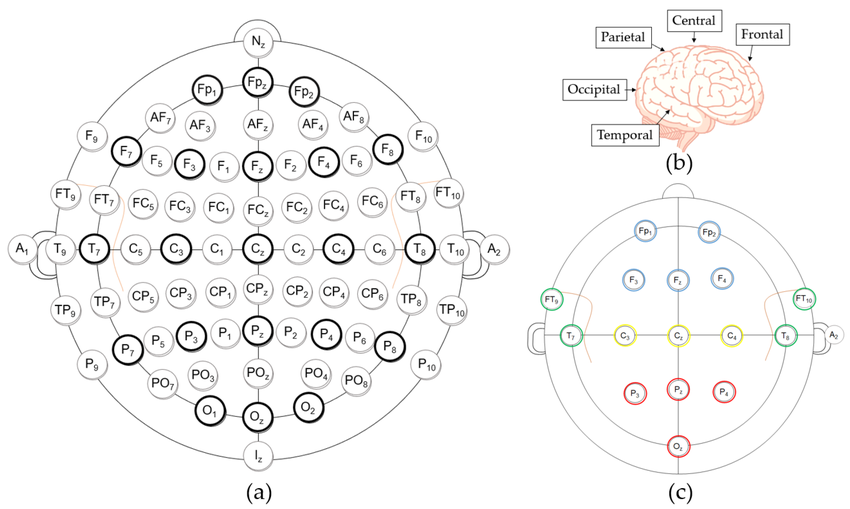
\includegraphics[width=1\textwidth]{Images/electrode-placement.png}
        \caption{(a) The 10-10 electrode placement system (Bold: 10–20 system); 
        (b) The cerebral lobes and central area; 
        (c) The placement configuration of the 16 electrodes.}

        \vspace{0.2cm}
        {\small \textit{Source:} Drowsiness Detection Based on Intelligent Systems with Nonlinear Features for Optimal Placement of Encephalogram Electrodes on the Cerebral Area - Scientific Figure on ResearchGate. Available from: \url{https://www.researchgate.net/figure/a-The-10-10-electrode-placement-system-Bold-10-20-system-b-The-cerebral-lobes-and_fig2_349257316} [accessed 12 Jan 2026]}
        \label{fig:electrode-placement}
    \end{figure}
    

    \subsection{Data Acquisition}
    While the headset provides recording functions, I am currently developing the custom data streaming pipeline to capture and synchronise these signals in real-time to control the game later on.
    \subsection{Summary}
    I have completed the initial hardware testing. The remaining 30\% of this phase involves finalising the streaming code and, most importantly, testing the Motor Imagery (MI) signals (the shifting experiment) to ensure the hardware can deliver the required functionality before proceeding to subsequent phases.

    

\chapter{Reflection \& Iteration}
    
    Reflecting on the progress against the Gantt chart, the project is currently slightly behind schedule.
    \begin{itemize}
        \item \textbf{Timeline Status:} I anticipated starting Phase 3 (Standard Protocol Dev) by this week. However, I am still concluding the final tasks of Phase 2.
        \item \textbf{Reason for Delay:} The technical investigation into the hardware constraints (specifically the electrode placement issue described in 1.3) required more time than anticipated. Devising the "positional shifting" strategy was necessary to ensure the project remains viable, but this research delayed the start of the software interface development.
        \item \textbf{Mitigation Strategy:} To recover the timeline, I will compress Phase 3. Rather than building a complex GUI for the Standard Protocol from scratch, I will utilise a simplified CLI (Command Line Interface) for data collection. This will allow me to recover lost time and align with the planned start of Phase 4 (Game Development).    

    \end{itemize}


    \begin{figure}[h]
        \centering
        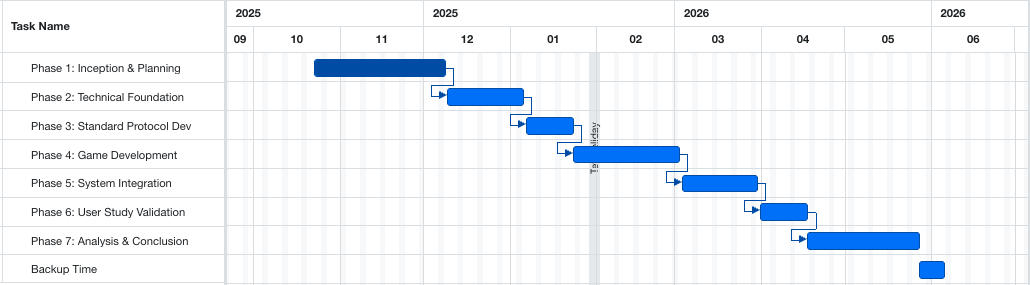
\includegraphics[width=1\textwidth]{Images/timeline.png}
        \caption{Initial Project Timeline}
        \label{fig:timeline}
    \end{figure}
    
\chapter{Action Plan}
    
    My immediate focus is to execute a rapid completion of Phase 2 to transition into Phase 3 without further delay.
    
    \section{Pipeline Completion}
    I will finalise the script to stream real-time raw data from the device by the end of this week.
    
    \section{MI Signal Verification}
    Concurrently, I will execute the Positional Shifting Experiment. I will record EEG data while performing motor tasks (hand clenching) with the position-adjusted headset. The objective is to explicitly confirm if Event-Related Desynchronisation (ERD) patterns are distinguishable.

    \section{Strategic Decision}
    \begin{itemize}
        \item Scenario A (Success): If ERD patterns are validated, I will proceed with the data collection protocol development as planned.
        \item Scenario B (Fallback): If clear motor signals cannot be detected, I will pivot to a Cognitive Control approach. Instead of motor commands, the game will be adapted to respond to Concentration (using Frontal EEG) and Stress (using PPG).
    \end{itemize}

\end{document}
